\chapter{Software Architecture and Implementation}
\label{chap:Software_Architecture_and_Implementation}

\section{Robot Operative System (ROS)}

In robotics, the amount of code required to get functional robots is quite big, since the coding goes from a driver level of the components to more higher level AI algorithms and routines. Usually, it is difficult to write code that can be adapted to several platforms or robots, and the persons in charge of this may have different choices of languages, depending on the expertise. These reasons make the integration of the different applications required to get the robot up and running a challenging work.\\

ROS is a response to these necessities, and the result is an meta-operative system designed to build a framework that provides an abstract communication layer between robotic applications in order to minimize integration efforts and reuse code. This will allow to use the same program with different platforms, accross different languages and different levels of the software, simplifying a lot the work required to develop an experimental set and making it possible to expand easily the experiments. ROS can also run in a distributed way, so that different processes can run in different computers accross a Local Area Network (LAN) \cite{Quigley}.\\

The ROS architecture is built in a peer-to-peer topology, where a number of processes can be running in a single host or in several hosts and communicate to each other. The coordination of the communication tasks is done by a \emph{master} process that can run in any computer in the network. The ability to run several nodes in different languages is achieved by a language-neutral interface definition language (IDL), that specifies each field of the message for the code generators and compilers of each language to generate an implementation native to the correspondent language. 

\subsection{Nomenclature}

ROS functionality can be distributed in the following elements:

\begin{itemize}

\item \textbf{Nodes} A node is any individual process in the system that performs a computational task. Nodes can be organized in a nested way, so a node can consist of several smaller nodes with distributed functionality. ROS can create a visual interface to see the organization of the currently running nodes with simple commands in the terminal.

\item \textbf{Messages} A message is the way that ROS nodes communicate between each other. It is a strictly typed data structure defined as a short text file for the compiler to interpret. A message can have primitive type like integers, doubles and floats; as well as other previously defined messages in a nested fashion.

\item \textbf{Topics} A node sends a message through topics. A topic is the channel that ROS provides to send and receive messages. A topic is defined by a string, such as "\emph{navigation}". When a node sends a message, it is said that the node has "\emph{published}" a message to a certain topic, and when it receives a message it does it by "\emph{subscribing}" to a certain topic.

\item \textbf{Services} In case of requiring syncronous communication between nodes, ROS offers services. A service consists of three elements: a string that defines the name and two strictly typed messages, one for the request and one for the response. Unlike topics, only one node can advertise a particular service with a unique name. 

\item \textbf{Parameter Server} This is a very useful resource that ROS provides. It stores variable values of different types and used for different purposes while ROS is up and running. Some of these variables can be parameters for the running applications or configuration settings. These parameters can be loaded each time through a \emph{launch} file and a configuration file written in YAML format \cite{Ben-kiki2004}. The launch file initiates ROS, specifies the nodes that should be running for a particular application, and loads the parameter server with the information provided by the YAML file. One big advantage of this way of launching nodes is that the configuration file does not need to be compiled each time, so one can change parameters without the downtime used compiling. 

\end{itemize}

\section{Library overview}

A quick description of the library can be made from Figure \ref{fig:inheritance_class_diagram} and Figure \ref{fig:implementation_class_diagram}. In Figure \ref{fig:inheritance_class_diagram}, the inheritance relationship between the interface classes and each particular instance of those classes can be seen directly here, without any functional relationship being displayed. The base classes are implemented with pure virtual functions or as interfaces; this is, they only exist through instances that inherit their methods and attributes. The interface classes cannot exist by themselves. The methods and attributes implemented in each particular application are the same, but particular implementation is defined in the derived objects.\\

The functional relation between the classes is displayed in Figure \ref{fig:implementation_class_diagram}. A particular instance of the ModelPredictiveControl interface class is responsible of solving the MPC problem, which unifies the functionality of the Model, Optimizer and Simulator (if any simulator is to be used; if not, the information is shared to the platform via ROS topic) classes.

\begin{figure}[H]
\centering
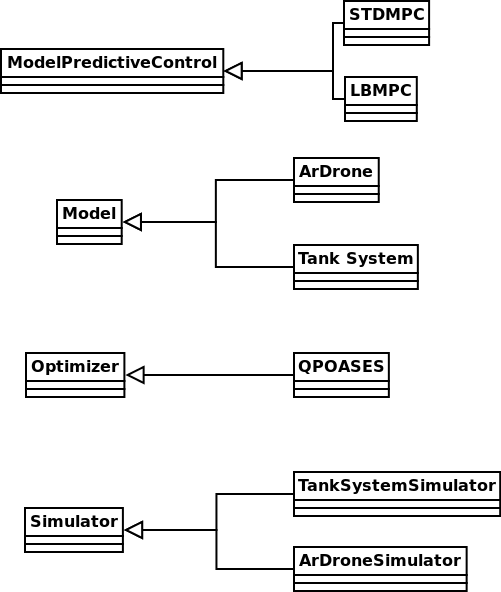
\includegraphics[scale=0.4]{Images/Chapter4/Class_Diagram.png}
\caption{Inheritance relationship between the interface and the implementation classes.}
\label{fig:inheritance_class_diagram}
\end{figure}

\begin{figure}[H]
\centering
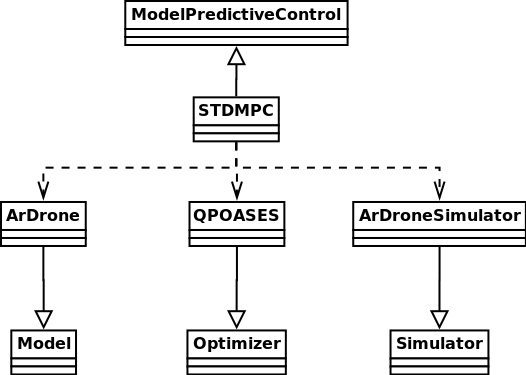
\includegraphics[scale=0.4]{Images/Chapter4/Class_diagram_implementation.png}
\caption{Implementation example of the class hierarchy for the ArDrone case.}
\label{fig:implementation_class_diagram}
\end{figure}

The main requirements for this library at the moment of its design were the following:

\begin{itemize}

\item \textbf{Expandability.} This software is thinked of so that users would know how to adapt the software easily to their specific applications with a small amount of modifications of the base program. The aim of the group is to be able to develop more functionality based on the foundational blocks of code that are created in this version. Since there are a lot of variants of the MPC algorithm, the goal is to be able to provide this options for the end user. 

\item \textbf{Modularity.} The software is designed to work with different quadratic programming solvers, different models and different simulators, just by creating derived classes from the bases that are provided. In this way, the possible combination of solvers, platforms and simulators is increased allowing for result verification and/or adapting the possible combinations to obtain the best performance for a particular application. This is also useful in order to allow to reuse code, since once a derived class for an application is completed it is ready to use in any other application available, which is why this feature is closely related to the previously mentioned expandability.

\end{itemize}

\section{Interface classes}

In this section is described in detail how each class works and integrates with each other and how they are built to achieve this goal. 

\subsection{Model}

The Model base class is used to provide the information of the dynamics of the desired model to the MPC solver. The model is provided as a linear state space model, as follows:

\begin{equation} \label{eq:model_representation}
\begin{cases}
\dot{\mathbf{x}} &= A\mathbf{x} + B\mathbf{u} \\
\mathbf{y} &= C\mathbf{x} + D\mathbf{u}
\end{cases}
\end{equation} 

So far, the only quadratic program solver that has been used provides support for models expressed in this form. If further development is continued, the aim is to provide support for the types of models that are mentioned in section \ref{impulsemodel1} and \ref{transferfunctionmodel1}.\\

The functionality of this class can be summarized in three simple actions: compute, set and get. The Model class \emph{computes} the system matrices, \emph{gets} the number of states, inputs and outputs; and \emph{sets} the states and inputs of the corresponding model.The header file provides a structure to build up upon, so that the user can define in the source file the specific information from the desired process model to be used and how these functions are being implemented. 

\begin{itemize}

\item computeDynamicModel function: this function takes the address of three Eigen matrix objects of the desired size and assigns the system matrices to those addresses as global variables for further use, returning a boolean variable to indicate success or failure. The matrices can be simply defined if the elements of each are known, or they can be calculated and discretized online when the function runs. These two ways are shown in the two different systems implemented in this thesis: in the case of the tank system, the matrices are just entered in the function so they are filled when the function runs; in the ARDrone quadrotor case, the matrices are calculated around the desired linearization point and discretized everytime the functions runs. The linearization and discretization methods are defined by the user, as long as a model with the previously mentioned structure is obtained.

\item getStatesNumber function: this function takes no inputs and returns an integer with the number of states defined by the user in the source file. The states number is stored as a global variable for further use.

\item getInputsNumber function: the same functionality as the previous get function, but with the number of inputs to the model.

\item getOutputsNumber function: the same functionality as the previous get function, but with the number of outputs of the model.

\item setStates function: this function takes an array of doubles as input and returns a boolean variable indicating success or failure at termination of the routine. The function assigns the elements of the array to the state vector array, so it is used for updating states at the end of the control loop.

\item setInputs function: this function has the same functionality as the previous set function, but with the inputs to the model.

\end{itemize}

As seen in Figure \ref{fig:implementation_class_diagram}, the Model interface class is one of the three classes that must be instantiated to be provided to an instance of the ModelPredictiveControl class to solve the MPC problem. The benefit of using an interface class is that any particular derived object can be instantiated as a pointer to the base class. This allows an easier integration between objects.

\subsection{Optimizer}

This interface class is designed to provide a way to integrate the selected quadratic programming solver to the MPC framework. Due to the variability of solvers and options available in each, this class was kept as simple as possible, to make it easier to adapt the functionality of the quadratic programming softwares and their individual options. The idea is to be able to adapt several solvers that use different methods to solve the quadratic problem depending on the structure of the problem and the particular application. \\

The integration of any solver is thinked of as a \emph{wrapper} or a frame to build upon the original functionality of the solver. The approach is to try to solve the quadratic problem including methods as simple and intuitive as possible in the class, so the details of the use of the specific solver are not required by the end user. To achieve that goal, the methods implemented were the following:

\begin{itemize}

\item init function: this function reads all the parameters required for the initialization and setting of the variables of the solver from ROS' parameter server. This function should be overloaded for each solver in particular.

\item computeOpt function: in this function the quadratic problem is solved. Several solvers require a "\emph{cold}" start run to get better approximations and improve the speed of the calculation, as is the case with qpOASES. In this particular case, it means that there are two different functions, one for the "\emph{cold}" start and one for the "\emph{hot}" start. The function recognizes this difference and launches the appropiate methods in each case. The results are stored in a protected global variable for the class. The exceptions thrown by the solver are also made easier to read and interpret for the end user, through messages that are visible in the terminal window.

\item getOptimalSolution function: this function is made to be used outside of the scope of the optimizer class instance, to be able to obtain the optimal solution, since they are protected inside the class.

\item getConstraintNumber function: this function is made to be used outside the scope of the optimizer class instance, to provide the number of constraints wherever needed.

\item getVariableNumber function: this function is made to be used outside the scope of the optimizer class instance, to provide the number of variables involved in the quadratic problem wherever needed.

\end{itemize}  

The methods of this class can be extended in the case that other software need more specific functionality. These are the functions that work with the chosen solver for this thesis, but there is a great interest of expansion in this direction to allow the user to decide which optimization algorithm suits best the application.

\subsection{Simulator}

This class is a frame for methods to simulate numerically a determined system. It works as a black-box: given some inputs and a sampling time, it delivers outputs. Since the idea is to replicate numerically as accurately as possible the behavior of the real system, the equations used in the simulator are the ones that provide the closest results to the outputs of the real system. Thus, in the quadrotor case, the equations being used to simulate are the ones from the non linear system. The functionality of this class is quite small, and it is all detailed in one single function:

\begin{itemize}

\item simulatePlant function: as described before, this function comprehends the whole functionality of the class. It takes as inputs arrays of double representing the current states, the control inputs and the sampling time; and it delivers as outputs the array of states for the next iteration. 

\end{itemize}

\subsection{ModelPredictiveControl}

This is the main class that unifies all the functionality of the previous ones to actually solve the quadratic problem posed by each MPC iteration. In the end, the methods from this class are the main methods to be used by the end user in the MPC implementation. This class also allows developers to work in their own variety of MPC, as they are a lot of varieties existing and also being developed. For example, there is currently ongoing work on developing a class to implement Learning Based Model Predictive Control, in which statistical learning algorithms are used to "learn" the non linearities and imperfections of the model and continue updating it as time goes by, thus allowing to reduce the initial modeling effort to obtain a model that is as accurate as possible. \\

All of these classes would have to adapt their main functionality to the following three methods to keep the ease of use of the library. Any additional functionality should be added in that particular class.

\begin{itemize}


\item resetMPC function: this function takes a pointer to an object of the Model, Optimizer and Simulator classes and sets the into the ModelPredictiveControl object, therefore providing the class with all the information and methods from these. Here is where the benefits of using interface classes comes into play: because of this, the pointers to the aforementioned objects can be instantiated as interface classes despite what object it is, as long as they are derived from them. This makes the implementation in the main function easily interchangeable between systems, solvers and simulators as longs as they are provided.

\item initMPC function: in this function all the parameters required to define the problem are read and all the initial calculations are performed. The parameters are read from ROS's parameter server, which can be modified without compiling afterwards using configuration files written in YAML format. This allows quick modifications without the time consuming compilation process.

\item updateMPC function: in this function is where the actual MPC problem is solved. The function takes the current state of the system and the desired reference for the system as inputs, and uses all the previously computed variables and parameters required to assemble the quadratic problem, then it summons the functionality from the optimizer class in order to solve the problem and provide a solution.   

\end{itemize}




